\documentclass[a4paper,12pt]{article}

% --- Подключение пакетов ---
\usepackage[T2A]{fontenc}
\usepackage[utf8]{inputenc}
\usepackage[russian]{babel}

\usepackage{amsmath}
\usepackage{amssymb}
\usepackage{amsfonts} % Мат. символы

\usepackage{graphicx} % Для вставки картинок
\usepackage{geometry} % Поля страницы
\usepackage{listings} % Для вставки кода
\usepackage{xcolor}   % Цвета для кода
\usepackage{hyperref} % Гиперссылки
\usepackage{multirow} % Для корректной компиляции таблицы
\usepackage{float}    % Плавающие объекты

% --- Настройка полей ---
\geometry{left=2cm, right=1.5cm, top=2cm, bottom=2cm}

% --- Авторская настройка для адекватной вставки кода с использованием кириллицы ---
\lstdefinestyle{mypython}{
    language=Python,
    basicstyle=\ttfamily\scriptsize,
    keywordstyle=\color{blue}\bfseries,
    stringstyle=\color{red},
    commentstyle=\color{green!60!black},
    numbers=left,
    numberstyle=\tiny\color{gray},
    stepnumber=1,
    numbersep=8pt,
    showspaces=false,
    showstringspaces=false,
    tabsize=4,
    frame=single,
    rulecolor=\color{black},
    breaklines=true,
    breakatwhitespace=false,
    captionpos=b,
    xleftmargin=15pt,
    xrightmargin=5pt,
    framexleftmargin=12pt,
    backgroundcolor=\color{gray!5},
    literate=%
        {а}{{\cyra}}1 {б}{{\cyrb}}1 {в}{{\cyrv}}1 {г}{{\cyrg}}1 {д}{{\cyrd}}1
        {е}{{\cyre}}1 {ё}{{\cyrie}}1 {ж}{{\cyrzh}}1 {з}{{\cyrz}}1 {и}{{\cyri}}1
        {й}{{\cyrishrt}}1 {к}{{\cyrk}}1 {л}{{\cyrl}}1 {м}{{\cyrm}}1 {н}{{\cyrn}}1
        {о}{{\cyro}}1 {п}{{\cyrp}}1 {р}{{\cyrr}}1 {с}{{\cyrs}}1 {т}{{\cyrt}}1
        {у}{{\cyru}}1 {ф}{{\cyrf}}1 {х}{{\cyrh}}1 {ц}{{\cyrc}}1 {ч}{{\cyrch}}1
        {ш}{{\cyrsh}}1 {щ}{{\cyrshch}}1 {ъ}{{\cyrhrdsn}}1 {ы}{{\cyrery}}1
        {ь}{{\cyrsftsn}}1 {э}{{\cyrerev}}1 {ю}{{\cyryu}}1 {я}{{\cyrya}}1
        {А}{{\CYRA}}1 {Б}{{\CYRB}}1 {В}{{\CYRV}}1 {Г}{{\CYRG}}1 {Д}{{\CYRD}}1
        {Е}{{\CYRE}}1 {Ё}{{\CYRIE}}1 {Ж}{{\CYRZH}}1 {З}{{\CYRZ}}1 {И}{{\CYRI}}1
        {Й}{{\CYRISHRT}}1 {К}{{\CYRK}}1 {Л}{{\CYRL}}1 {М}{{\CYRM}}1 {Н}{{\CYRN}}1
        {О}{{\CYRO}}1 {П}{{\CYRP}}1 {Р}{{\CYRR}}1 {С}{{\CYRS}}1 {Т}{{\CYRT}}1
        {У}{{\CYRU}}1 {Ф}{{\CYRF}}1 {Х}{{\CYRH}}1 {Ц}{{\CYRC}}1 {Ч}{{\CYRCH}}1
        {Ш}{{\CYRSH}}1 {Щ}{{\CYRSHCH}}1 {Ъ}{{\CYRHRDSN}}1 {Ы}{{\CYRERY}}1
        {Ь}{{\CYRSFTSN}}1 {Э}{{\CYREREV}}1 {Ю}{{\CYRYU}}1 {Я}{{\CYRYA}}1
}
\lstset{style=mypython}

\begin{document}

% ===========================================================================
% 1. ТИТУЛЬНЫЙ ЛИСТ
% ===========================================================================
\begin{titlepage}
    \centering
    % Шапка
    {\fontsize{11}{13}\selectfont \textbf{Министерство науки и высшего образования Российской Федерации}} \\
    {\fontsize{7}{10}\selectfont ФЕДЕРАЛЬНОЕ ГОСУДАРСТВЕННОЕ АВТОНОМНОЕ ОБРАЗОВАТЕЛЬНОЕ УЧРЕЖДЕНИЕ ВЫСШЕГО ОБРАЗОВАНИЯ} \\
    \vspace{0.2cm} 
    {\fontsize{14}{17}\selectfont \textbf{«НАЦИОНАЛЬНЫЙ ИССЛЕДОВАТЕЛЬСКИЙ УНИВЕРСИТЕТ ИТМО»}}
    
    \vspace{1cm} 
    
    % Информация о группе
    {\fontsize{12}{14}\selectfont \textbf{Группа P3211}}
    
    \vspace{1cm}
    
    % Информация о дисциплине
    {\fontsize{12}{14}\selectfont \textbf{Дисциплина: Математическая статистика}}
    
    \vspace*{\fill}
    
    % Заголовок работы
    {\fontsize{18}{22}\selectfont \textbf{РАСЧЁТНО-ГРАФИЧЕСКАЯ РАБОТА №1}} \\
    \vspace{0.5cm}
    {\fontsize{14}{17}\selectfont \textbf{по теме: «Описание выборки. Оценивание параметров. Доверительные интервалы»}}
    
    \vspace{2cm}
    
    {\fontsize{12}{14}\selectfont \textbf{Вариант A-10}}
    
    \vspace{2cm}
    
    % Блок выполнил/проверил
    \begin{flushright}
        \fontsize{12}{14}\selectfont
        Выполнил: \\
        Михайлов Петр Сергеевич \\
        Гришин Артем Евгеньевич \\
        \vspace{1em}
        Преподаватель: \\
        Селина Елена Георгиевна
    \end{flushright}
    
    \vfill
    
    % Подвал
    {\fontsize{12}{14}\selectfont
    Санкт-Петербург, 2026
    }
\end{titlepage}

\setcounter{page}{2}

\newpage

% ===========================================================================
% 2. Оглавление
% ===========================================================================
\tableofcontents

\newpage

% ===========================================================================
% 3. Основная обязательная часть
% ===========================================================================

\section{Первичное описание выборки (пункт 4.1)}

В рамках данной работы исследуются три случайные величины $X_1, X_2, X_3$ объемом $n=200$ каждая.

\subsection{Вариационный ряд и экстремальные значения}
Для каждой выборки был построен вариационный ряд $x_{(1)} \le x_{(2)} \le \dots \le x_{(n)}$. 
\begin{itemize}
    \item $X_1$: Минимум $x_{(1)} \approx 12.02$, Максимум $x_{(n)} \approx 394.28$
    \item $X_2$: Минимум $x_{(1)} \approx 7.71$, Максимум $x_{(n)} \approx 58.95$
    \item $X_3$: Минимум $x_{(1)} \approx 30.47$, Максимум $x_{(n)} \approx 78.66$
\end{itemize}

Ниже код для составления вариационного ряда:
\begin{lstlisting}[language=Python, caption={Содержание файла 1\_variational\_series.py}]
import pandas as pd

df = pd.read_csv('RGR1_A-10_X1-X4.csv')
columns = ['X1', 'X2', 'X3']

print("=== Вариационные ряды ===")
for col in columns:
    # Сортировка данных по возрастанию
    var_series = df[col].sort_values().reset_index(drop=True)
    
    print(f"\nСтолбец {col}:")
    print(f"Минимум: {var_series.iloc[0]}, Максимум: {var_series.iloc[-1]}")
    print(f"Первые 5 элементов:\n{var_series.head()}")
    print(f"Последние 5 элементов:\n{var_series.tail()}")
    
    # var_series.to_csv(f'var_series_{col}.txt', index=False, header=False)
\end{lstlisting}

\newpage

\begin{figure}[H]
    \centering
    \includegraphics[width=0.5\textwidth]{vyvod_1.png}
    \caption{Вывод кода}
    \label{fig:ecdf}
\end{figure}

\subsection{Эмпирическая функция распределения}
Ниже представлены графики эмпирической функции распределения $F_n(x)$ для исследуемых величин.

\begin{figure}[H]
    \centering
    \includegraphics[width=0.9\textwidth]{ecdf_plots.png}
    \caption{Эмпирические функции распределения для $X_1, X_2, X_3$}
    \label{fig:ecdf}
\end{figure}

\subsection{Гистограммы и правила группировки}
Для визуализации плотности распределения были построены гистограммы с использованием трех различных правил выбора количества интервалов ($k$):

\begin{enumerate}
    \item \textbf{Правило Стерджеса:} $k = 1 + \lfloor \log_2 n \rfloor$. Наиболее грубое правило, часто дает слишком широкие интервалы для больших выборок.
    \item \textbf{Правило Скотта:} $h = 3.5 \hat{\sigma} n^{-1/3}$. Учитывает разброс данных через стандартное отклонение.
    \item \textbf{Правило Фридмана-Диакониса:} $h = 2 IQR n^{-1/3}$. Наиболее устойчивое к выбросам правило, так как использует межквартильный размах.
\end{enumerate}

\begin{figure}[H]
    \centering
    \includegraphics[width=0.8\textwidth]{hist_sturges.png}
    \caption{Гистограммы по правилу Стерджеса}
\end{figure}

\begin{figure}[H]
    \centering
    \includegraphics[width=0.8\textwidth]{hist_scott.png}
    \caption{Гистограммы по правилу Скотта}
\end{figure}

\begin{figure}[H]
    \centering
    \includegraphics[width=0.8\textwidth]{hist_fd.png}
    \caption{Гистограммы по правилу Фридмана-Диакониса}
\end{figure}

\textbf{Сравнение результатов:}
Анализ гистограмм показывает, что для данных выборок правило Стерджеса дает наиболее сглаженный вид, в то время как правило Фридмана-Диакониса лучше детализирует особенности распределения (особенно заметно на $X_2$, где проявляется «П-образная» форма). Правило Скотта занимает промежуточное положение.

\subsection{Числовые характеристики}
Ниже представлены результаты расчета числовых характеристик выборки (вывод скрипта \texttt{6\_numerical\_characteristics.py}):

\begin{figure}[H]
    \centering
    % Вставь сюда скриншот консоли или таблицу с результатами
    \includegraphics[width=0.7\textwidth]{vyvod_2.png} 
    \caption{Числовые характеристики выборок $X_1, X_2, X_3$}
\end{figure}

\subsection{Анализ формы распределения}
Согласно пункту 4.1.5, на основе визуального анализа гистограмм, ЭФР и вычисленных числовых характеристик, форму распределений можно описать следующим образом:
\begin{itemize}
    \item \textbf{Выборка $X_1$:} Наблюдается ярко выраженная правосторонняя асимметрия. Присутствуют выбросы в правой части распределения (формируется длинный «хвост» значений, достигающих 394.28 при медиане около 67). Имеется естественная левая граница (значения не опускаются ниже $\approx 12$), правая естественная граница отсутствует.
    \item \textbf{Выборка $X_2$:} Распределение в целом симметрично, гистограмма имеет вид, близкий к прямоугольному. Аномальные выбросы визуально и статистически отсутствуют. Присутствуют жесткие естественные границы как слева, так и справа — основная масса значений равномерно распределена строго внутри интервала от минимального до максимального значения.
    \item \textbf{Выборка $X_3$:} Распределение симметрично относительно центральной оси. Явных аномальных выбросов не наблюдается (основная масса значений плотно сконцентрирована вокруг центра). Теоретически естественные границы отсутствуют (значения могут принимать любые величины), но на практике они ограничены естественным затуханием плотности по краям.
\end{itemize}

\newpage

\section{Предположение о виде закона распределения (пункт 4.2)}

На основе анализа гистограмм, эмпирических функций распределения (ЭФР) и числовых характеристик, для каждого столбца выбрана наиболее подходящая теоретическая модель.

\textbf{1. Выборка $X_1$ — Экспоненциальное распределение со сдвигом ($\text{Exp}_{\lambda, c}$)}

Гистограмма демонстрирует характерное резкое убывание плотности с ростом значения признака, что свидетельствует о сильной асимметрии. ЭФР сначала круто возрастает, а затем постепенно выходит на плато. Кроме того, выборка имеет жесткую левую границу (значения строго больше нуля и начинаются с определенного порога $c$), а выборочное среднее заметно сдвинуто вправо относительно медианы из-за длинного «хвоста» больших значений.

\textbf{2. Выборка $X_2$ — Равномерное распределение ($U_{a, b}$)}

Гистограмма показывает примерно одинаковую частоту попадания значений в различные интервалы, образуя «П-образную» фигуру. График ЭФР на основном участке растет практически линейно, без резких изгибов. Выборочное среднее и медиана близки друг к другу, а сами данные строго ограничены минимальным и максимальным значениями (естественными границами $a$ и $b$) без затухающих «хвостов» на краях.

\textbf{3. Выборка $X_3$ — Нормальное распределение ($N_{a, \sigma}$)}

Гистограмма имеет классическую симметричную колоколообразную форму с выраженным максимумом в центре распределения. График ЭФР представляет собой характерную плавную S-образную кривую. Выборочное среднее практически полностью совпадает с медианой, что подтверждает симметричность распределения, а убывание частот по краям характерно для гауссовской кривой.

\newpage

\section{Оценивание параметров: метод моментов и метод максимального правдоподобия (пункт 4.3)}

В данном разделе для выбранных моделей распределений производится оценка параметров двумя способами. Метод моментов (ММ) основан на приравнивании теоретических моментов (математического ожидания $EX$ и дисперсии $DX$) к соответствующим выборочным оценкам $\overline{x}$ и $S^2$. Метод максимального правдоподобия (ММП) заключается в поиске значений параметров, максимизирующих функцию правдоподобия $L(\theta)$.

\subsection*{Общий принцип метода максимального правдоподобия}

Пусть $x_1, x_2, \dots, x_n$ --- выборка независимых, одинаково распределенных случайных величин с плотностью распределения $f(x, \theta)$, где $\theta$ --- неизвестный параметр. 

Совместная плотность распределения выборки, рассматриваемая как функция параметра $\theta$ при фиксированных значениях данных, называется \textbf{функцией правдоподобия}:
\[
L(\theta) = L(x_1, \dots, x_n; \theta) = \prod_{i=1}^{n} f(x_i, \theta)
\]
Поскольку функция $\ln(x)$ монотонно возрастает, точка максимума $L(\theta)$ совпадает с точкой максимума \textbf{логарифмической функции правдоподобия}:
\[
l(\theta) = \ln L(\theta) = \sum_{i=1}^{n} \ln f(x_i, \theta)
\]
Оценка максимального правдоподобия (ОМП) $\hat{\theta}_{ML}$ определяется как значение, доставляющее максимум этой функции:
\[
\hat{\theta}_{ML} = \arg\max_{\theta} L(\theta)
\]
В случаях, когда функция правдоподобия дифференцируема по $\theta$, оценка находится из системы уравнений правдоподобия:
\[
\frac{\partial l(\theta)}{\partial \theta_j} = 0
\]
Ниже приведены конкретные реализации данного принципа для исследуемых выборок.

\subsection*{Для выборки $X_1$ (Экспоненциальное распределение со сдвигом $\text{Exp}_{\lambda,c}$)}

Теоретические моменты: $EX = c + \frac{1}{\lambda}$, $DX = \frac{1}{\lambda^2}$.

\textbf{1. Метод моментов:}\\
Составляем систему уравнений:
$$
\begin{cases}
c + \frac{1}{\lambda} = \overline{x} \\
\frac{1}{\lambda^2} = S^2
\end{cases}
$$
Из второго уравнения получаем $\hat{\lambda}_{MM} = \frac{1}{S}$. Подставляя в первое уравнение, находим $\hat{c}_{MM} = \overline{x} - \frac{1}{\hat{\lambda}_{MM}} = \overline{x} - S$.

\textbf{2. Метод максимального правдоподобия:}\\
Функция правдоподобия имеет вид:
$$
L(\lambda,c) = \lambda^n e^{-\lambda\sum_{i=1}^{n}(x_i-c)}, \quad \text{при } c \le \min(X) = x_{(1)}
$$
При фиксированном $\lambda > 0$, функция $L(\lambda,c)$ монотонно возрастает по $c$. Следовательно, максимум достигается при наибольшем возможном $c$, удовлетворяющем условию $c \le x_{(1)}$. Отсюда:
$$
\hat{c}_{ML} = x_{(1)}
$$
Подставим $\hat{c}_{ML}$ в логарифмическую функцию правдоподобия и максимизируем по $\lambda$:
$$
\ell(\lambda) = \ln L(\lambda, \hat{c}_{ML}) = n\ln\lambda - \lambda\sum_{i=1}^{n}(x_i - \hat{c}_{ML})
$$
Дифференцируя по $\lambda$ и приравнивая производную к нулю:
$$
\frac{\partial\ell}{\partial\lambda} = \frac{n}{\lambda} - \sum_{i=1}^{n}(x_i - \hat{c}_{ML}) = 0 \quad \implies \quad \hat{\lambda}_{ML} = \frac{n}{\sum_{i=1}^{n}(x_i - \hat{c}_{ML})} = \frac{1}{\overline{x} - \hat{c}_{ML}}
$$

\subsection*{Для выборки $X_2$ (Равномерное распределение $U_{a,b}$)}

Теоретические моменты: $EX = \frac{a+b}{2}$, $DX = \frac{(b-a)^2}{12}$.

\textbf{1. Метод моментов:}\\
Составляем систему уравнений:
$$
\begin{cases}
\frac{a+b}{2} = \overline{x} \\
\frac{(b-a)^2}{12} = S^2
\end{cases}
$$
Решая систему, получаем: $b-a = \sqrt{12S^2} = 2S\sqrt{3}$. Отсюда:
$$
\hat{a}_{MM} = \overline{x} - S\sqrt{3}, \quad \hat{b}_{MM} = \overline{x} + S\sqrt{3}
$$

\textbf{2. Метод максимального правдоподобия}

Плотность равномерного распределения имеет вид:
\[ f(x|a,b) = \frac{1}{b-a} \cdot I_{[a, b]}(x) \]
где $I_{[a, b]}(x)$ --- индикаторная функция, равная $1$, если $x \in [a, b]$, и $0$ в противном случае. 

Тогда функция правдоподобия для выборки $x_1, \dots, x_n$ записывается как:
\[ L(a, b) = \prod_{i=1}^{n} \frac{1}{b-a} I_{[a, b]}(x_i) = \frac{1}{(b-a)^n} \prod_{i=1}^{n} I_{[a, b]}(x_i) \]

Произведение индикаторов равно единице только тогда, когда \textbf{все} элементы выборки лежат внутри отрезка $[a, b]$, что эквивалентно условию:
\[ a \le \min(x_i) \quad \text{и} \quad b \ge \max(x_i) \]

Следовательно, функция $L(a, b)$ отлична от нуля только при $a \le x_{(1)}$ и $b \ge x_{(n)}$. Чтобы максимизировать $L(a, b) = (b-a)^{-n}$, необходимо минимизировать длину интервала $(b-a)$. Это достигается при максимально возможном $a$ и минимально возможном $b$ в рамках заданных ограничений:
\[ \hat{a}_{ML} = x_{(1)} = \min\{x_1, \dots, x_n\}, \quad \hat{b}_{ML} = x_{(n)} = \max\{x_1, \dots, x_n\} \]

\subsection*{Для выборки $X_3$ (Нормальное распределение $N_{a, \sigma}$)}

Теоретические моменты: $EX = a$, $DX = \sigma^2$.

\textbf{1. Метод моментов:}\\
Приравнивая теоретические моменты к выборочным характеристикам, получаем систему уравнений:
$$
\begin{cases}
a = \overline{x} \\
\sigma^2 = S^2
\end{cases}
\implies \quad \hat{a}_{MM} = \overline{x}, \quad \hat{\sigma}_{MM} = S
$$

\textbf{2. Метод максимального правдоподобия:}\\
Плотность нормального распределения: $f(x|a,\sigma) = \frac{1}{\sigma\sqrt{2\pi}} e^{-\frac{(x-a)^2}{2\sigma^2}}$.\\
Логарифмическая функция правдоподобия:
$$
\ell(a,\sigma) = \ln L(a, \sigma) = -n \ln(\sigma\sqrt{2\pi}) - \frac{1}{2\sigma^2}\sum_{i=1}^{n}(x_i-a)^2
$$
Дифференцируя по $a$ и $\sigma$ (или $\sigma^2$) и приравнивая к нулю, получаем известные оценки:
$$
\hat{a}_{ML} = \overline{x}, \quad \hat{\sigma}_{ML}^2 = \frac{1}{n}\sum_{i=1}^{n}(x_i-\overline{x})^2 = S^2
$$
Таким образом, для нормального распределения оценки ММ и ММП совпадают.

\subsection{Численное сравнение оценок ММ и ММП}

Результаты вычислений с уточненными значениями представлены в таблице \ref{tab:estimates}.

\begin{table}[H]
\centering
\begin{tabular}{|c|c|c|c|c|}
\hline
Выборка & Параметр & Оценка ММ & Оценка ММП & Абсолютное расхождение \\ \hline
\multirow{2}{*}{$X_1$} & $\lambda$ & $\hat{\lambda}_{MM} = 0.0120$ & $\hat{\lambda}_{ML} = 0.0117$ & $2.3673 \cdot 10^{-4}$ \\
                       & $c$       & $\hat{c}_{MM} = 13.7024$      & $\hat{c}_{ML} = 12.0200$      & $1.6824$ \\ \hline
\multirow{2}{*}{$X_2$} & $a$       & $\hat{a}_{MM} = 36.5138$      & $\hat{a}_{ML} = 36.5138$      & $0.0000$ \\
                       & $\sigma$  & $\hat{\sigma}_{MM} = 9.3316$  & $\hat{\sigma}_{ML} = 9.3316$  & $0.0000$ \\ \hline
\multirow{2}{*}{$X_3$} & $a$       & $\hat{a}_{MM} = 29.7027$      & $\hat{a}_{ML} = 30.4700$      & $0.76727$ \\
                       & $b$       & $\hat{b}_{MM} = 78.4526$      & $\hat{b}_{ML} = 78.6600$      & $0.20743$ \\ \hline
\end{tabular}
\caption{Сравнение оценок метода моментов и метода максимального правдоподобия}
\label{tab:estimates}
\end{table}

\textbf{Комментарий к результатам:}
\begin{itemize}
    \item \textbf{Для нормального распределения ($X_2$):} Наблюдается полное совпадение оценок параметров $a$ (мат. ожидание) и $\sigma$ (стандартное отклонение). Это подтверждает теоретический факт: для нормального закона точечные оценки по обоим методам математически эквивалентны.
    
    \item \textbf{Для равномерного распределения ($X_3$):} Между ММ и ММП есть расхождение. Метод максимального правдоподобия оценивает границы $a$ и $b$ через крайние значения выборки ($x_{(1)}$ и $x_{(n)}$), что делает их более чувствительными к конкретным реализациям на границах. Метод моментов вычисляет их усредненно через разброс (дисперсию), что в данном случае дало отклонение порядка $0.76$ для левой границы.
    
    \item \textbf{Для экспоненциального распределения со сдвигом ($X_1$):} Расхождение наиболее выражено в параметре сдвига $c$ (разница $1.6824$). ММП жестко фиксирует $c$ на уровне минимального наблюдаемого значения $x_{(1)} = 12.02$. Оценка ММ ($13.7024$) оказывается выше, так как она зависит от баланса между средним арифметическим и стандартным отклонением, которые для этой выборки «тянут» оценку сдвига вправо.
\end{itemize}

\begin{figure}[H]
    \centering
    \includegraphics[width=0.9\textwidth]{vyvod_3.png} 
    \caption{Результаты работы скрипта 7\_estimates\_calculation.py}
    \label{fig:results_7}
\end{figure}

\newpage

Ниже приведен исходный код программы, использованной для автоматизации расчетов:

\begin{lstlisting}[style=mypython, caption={Содержание файла 7\_estimates\_calculation.py}]
import pandas as pd
import numpy as np

# Загрузка данных
df = pd.read_csv('RGR1_A-10_X1-X4.csv')

def calculate_estimates(data, name):
    n = len(data)
    mean_x = data.mean()
    s_std = data.std(ddof=0) # Смещенное СКО (как в ММП)
    min_x = data.min()
    max_x = data.max()

    results = {}

    if name == 'X1':  # Exp(lambda, c)
        # Метод моментов
        results['lambda_mm'] = 1 / s_std
        results['c_mm'] = mean_x - s_std
        # ММП
        results['c_ml'] = min_x
        results['lambda_ml'] = 1 / (mean_x - min_x)
        
    elif name == 'X2':  # N(a, sigma)
        # Метод моментов
        results['a_mm'] = mean_x
        results['sigma_mm'] = s_std
        # ММП
        results['a_ml'] = mean_x
        results['sigma_ml'] = s_std
        
    elif name == 'X3':  # U(a, b)
        # Метод моментов
        results['a_mm'] = mean_x - np.sqrt(3) * s_std
        results['b_mm'] = mean_x + np.sqrt(3) * s_std
        # ММП
        results['a_ml'] = min_x
        results['b_ml'] = max_x

    return results

print(f"{'Выборка':<8} | {'Параметр':<10} | {'Оценка ММ':<12} | {'Оценка ММП':<12} | {'Абс. расх.':<12}")
print("-" * 65)

for col in ['X1', 'X2', 'X3']:
    est = calculate_estimates(df[col], col)
    
    if col == 'X1':
        p1, p2 = 'lambda', 'c'
        m1_mm, m1_ml = est['lambda_mm'], est['lambda_ml']
        m2_mm, m2_ml = est['c_mm'], est['c_ml']
    elif col == 'X2':
        p1, p2 = 'a', 'sigma'
        m1_mm, m1_ml = est['a_mm'], est['a_ml']
        m2_mm, m2_ml = est['sigma_mm'], est['sigma_ml']
    else: # X3
        p1, p2 = 'a', 'b'
        m1_mm, m1_ml = est['a_mm'], est['a_ml']
        m2_mm, m2_ml = est['b_mm'], est['b_ml']

    diff1 = abs(m1_mm - m1_ml)
    diff2 = abs(m2_mm - m2_ml)

    print(f"{col:<8} | {p1:<10} | {m1_mm:<12.4f} | {m1_ml:<12.4f} | {diff1:<12.4e}")
    print(f"{'':<8} | {p2:<10} | {m2_mm:<12.4f} | {m2_ml:<12.4f} | {diff2:<12.4e}")
    print("-" * 65)
\end{lstlisting}

\newpage

\subsection{Визуализация результатов оценивания}

В данном подразделе приведены графики, визуализирующие результаты точечного оценивания параметров выборок методом моментов и методом максимального правдоподобия. Для каждой выборки построены:
\begin{enumerate}
    \item Сравнение нормированной гистограммы данных с теоретическими кривыми плотности распределения, построенными на основе полученных оценок ММ и ММП.
    \item Диаграмма размаха («ящик с усами») для анализа квартилей распределения, наличия выбросов и общей симметрии выборки.
\end{enumerate}

% --- Графики для X1 ---
\begin{figure}[H]
    \centering
    \begin{minipage}[b]{0.48\textwidth}
        \centering
        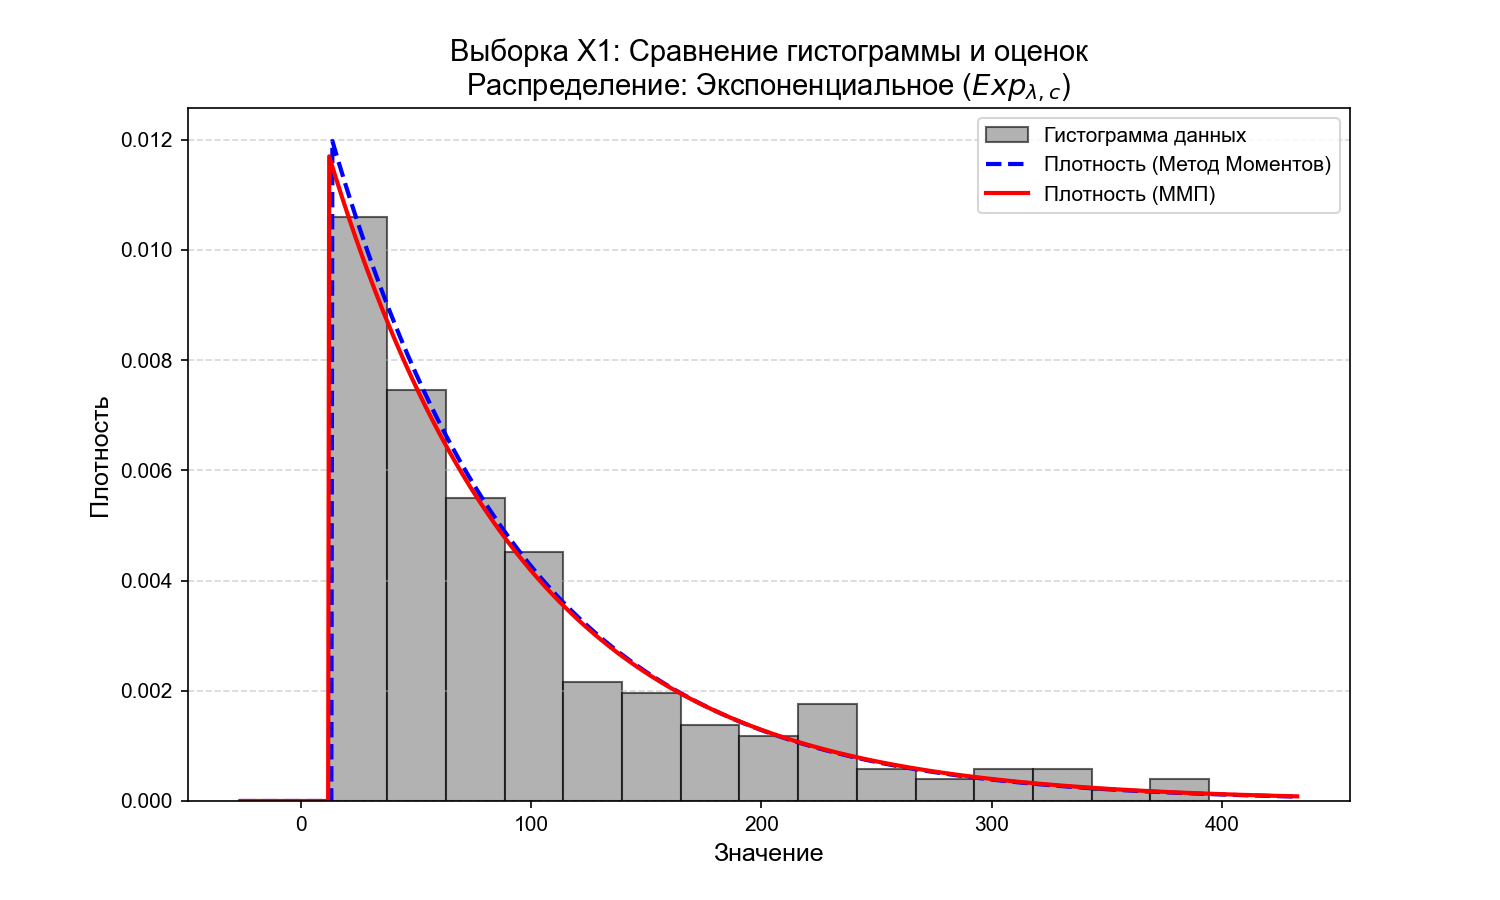
\includegraphics[width=\textwidth]{fit_comparison_X1.png}
        \caption{Выборка $X_1$: Сравнение гистограммы и оцененных плотностей ($Exp_{\lambda, c}$)}
    \end{minipage}
    \hfill
    \begin{minipage}[b]{0.48\textwidth}
        \centering
        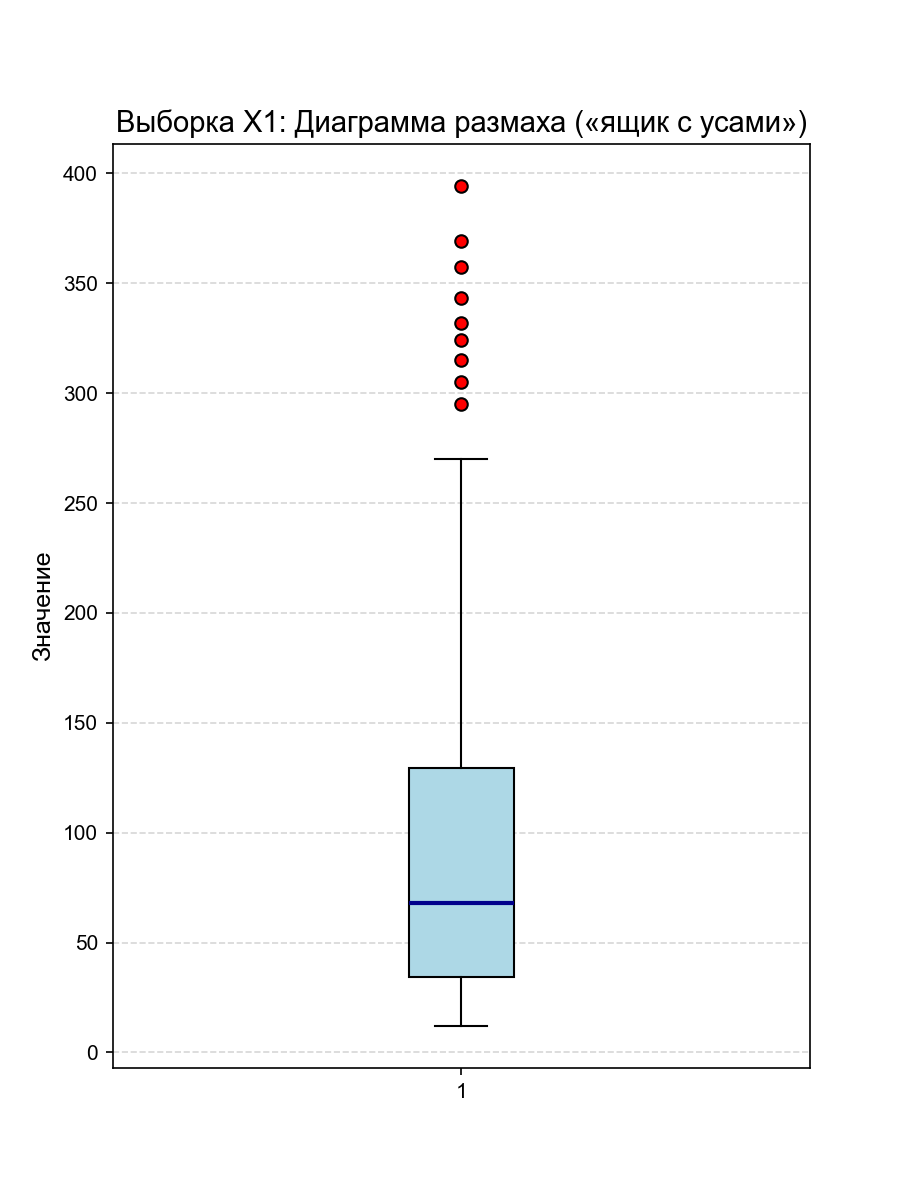
\includegraphics[width=0.75\textwidth]{boxplot_X1.png} % Ящик чуть уже
        \caption{Выборка $X_1$: Диаграмма размаха}
    \end{minipage}
\end{figure}

% --- Графики для X2 ---
\begin{figure}[H]
    \centering
    \begin{minipage}[b]{0.48\textwidth}
        \centering
        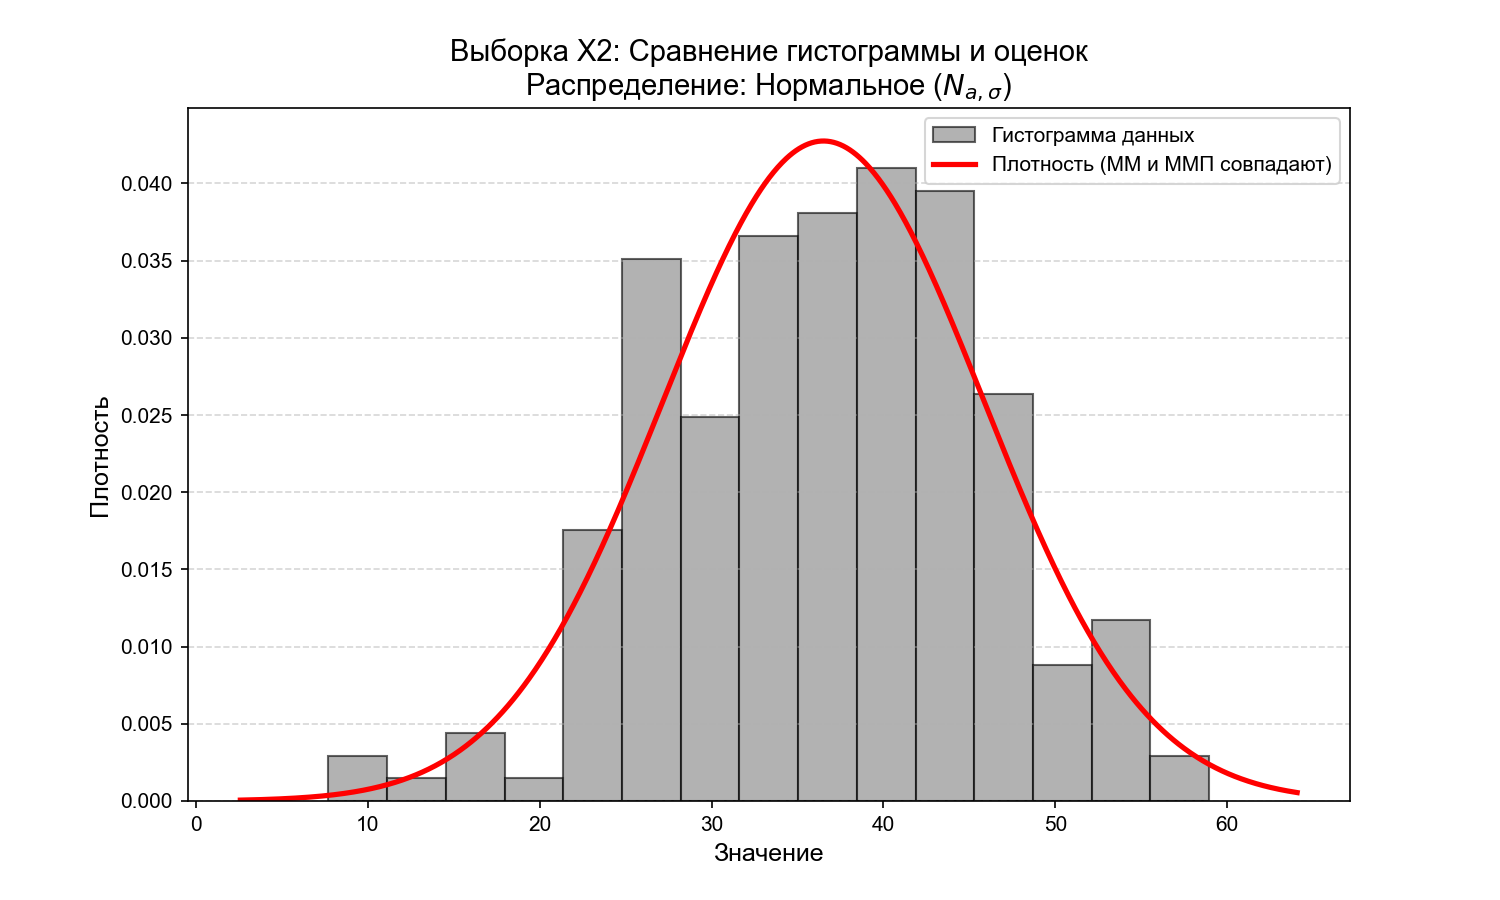
\includegraphics[width=\textwidth]{fit_comparison_X2.png}
        \caption{Выборка $X_2$: Сравнение гистограммы и оцененных плотностей ($N_{a, \sigma}$)}
    \end{minipage}
    \hfill
    \begin{minipage}[b]{0.48\textwidth}
        \centering
        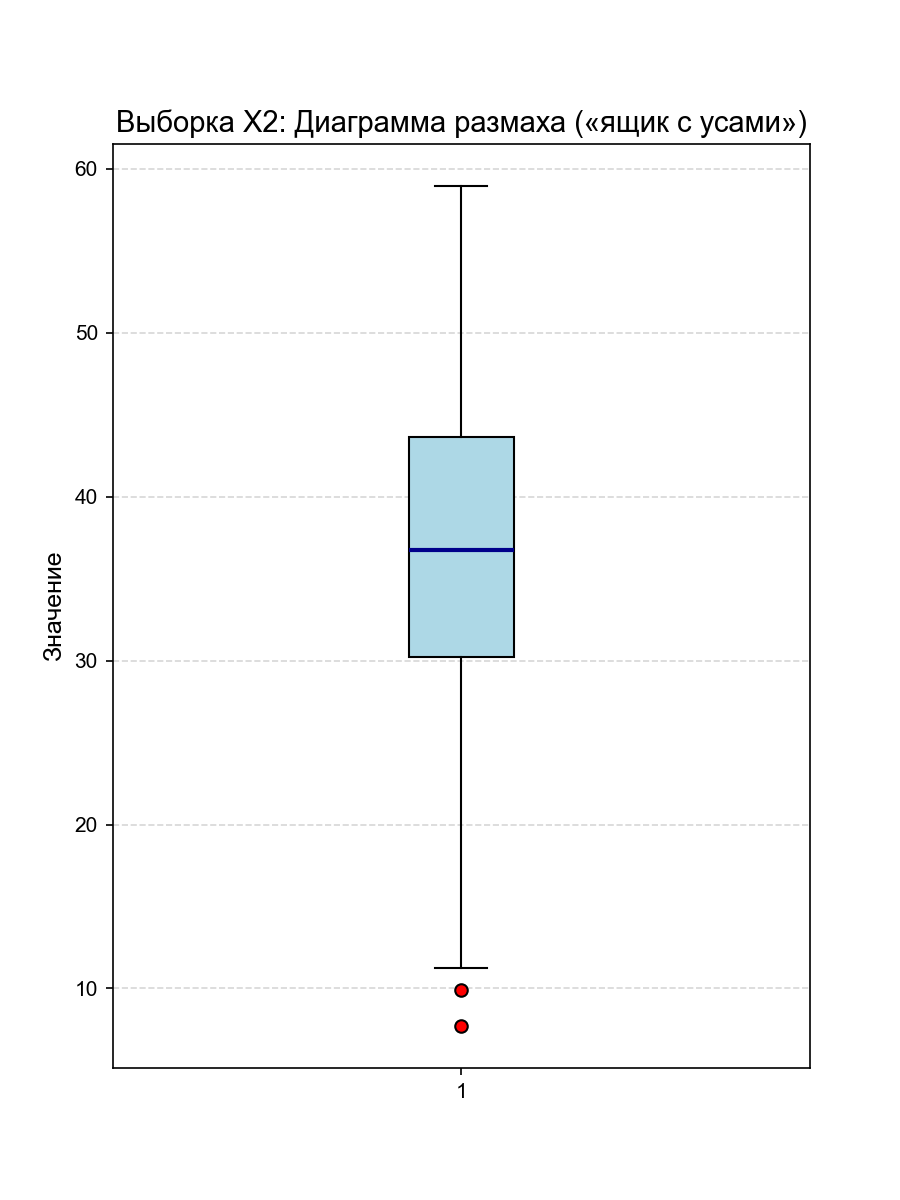
\includegraphics[width=0.75\textwidth]{boxplot_X2.png}
        \caption{Выборка $X_2$: Диаграмма размаха}
    \end{minipage}
\end{figure}

% --- Графики для X3 ---
\begin{figure}[H]
    \centering
    \begin{minipage}[b]{0.48\textwidth}
        \centering
        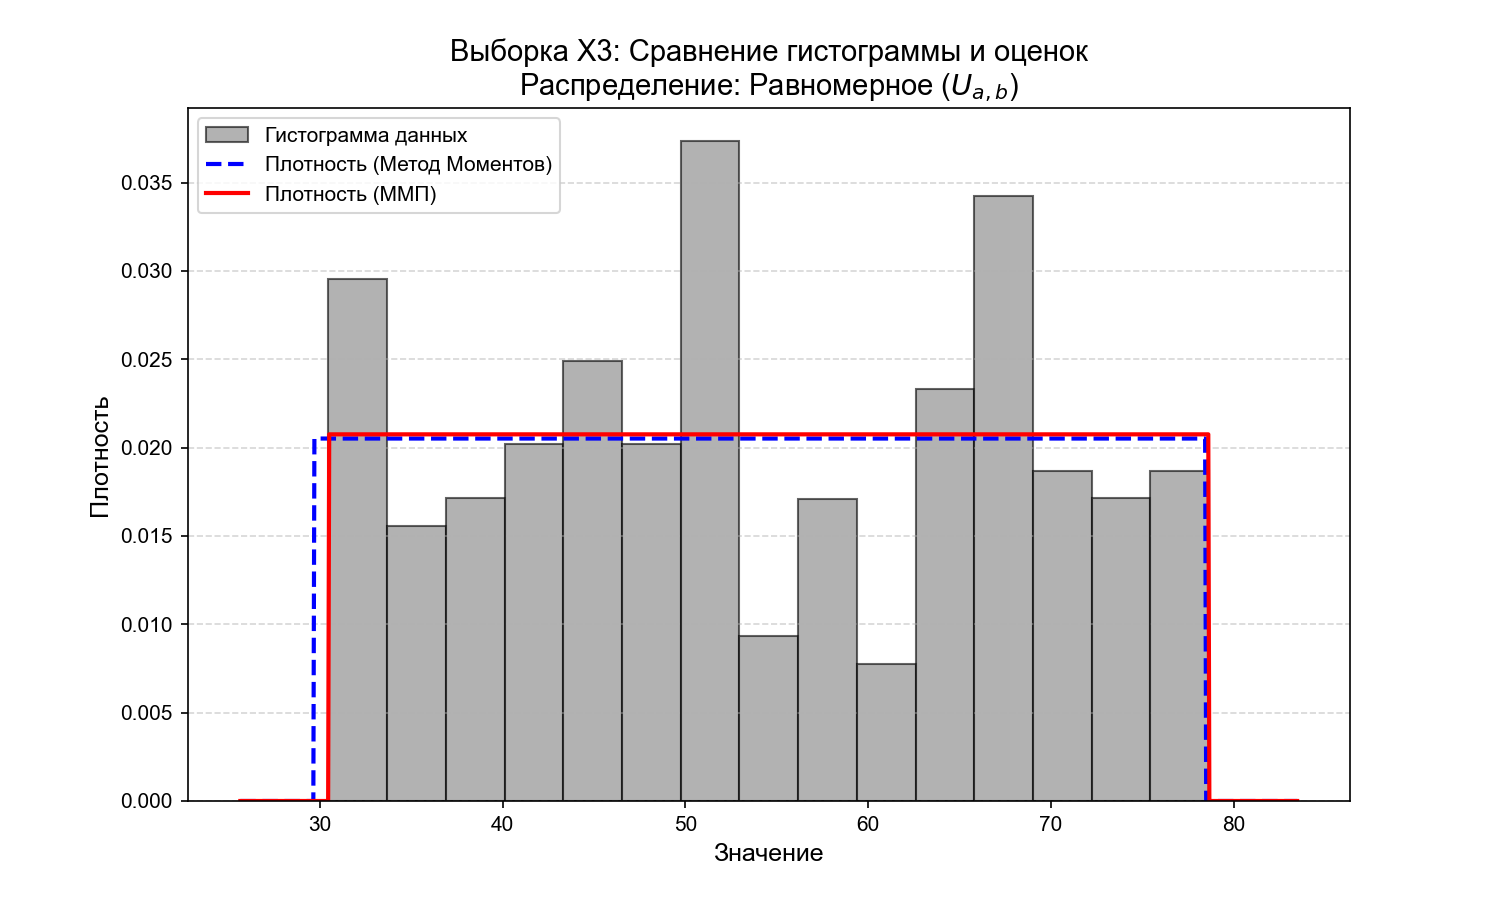
\includegraphics[width=\textwidth]{fit_comparison_X3.png}
        \caption{Выборка $X_3$: Сравнение гистограммы и оцененных плотностей ($U_{a, b}$)}
    \end{minipage}
    \hfill
    \begin{minipage}[b]{0.48\textwidth}
        \centering
        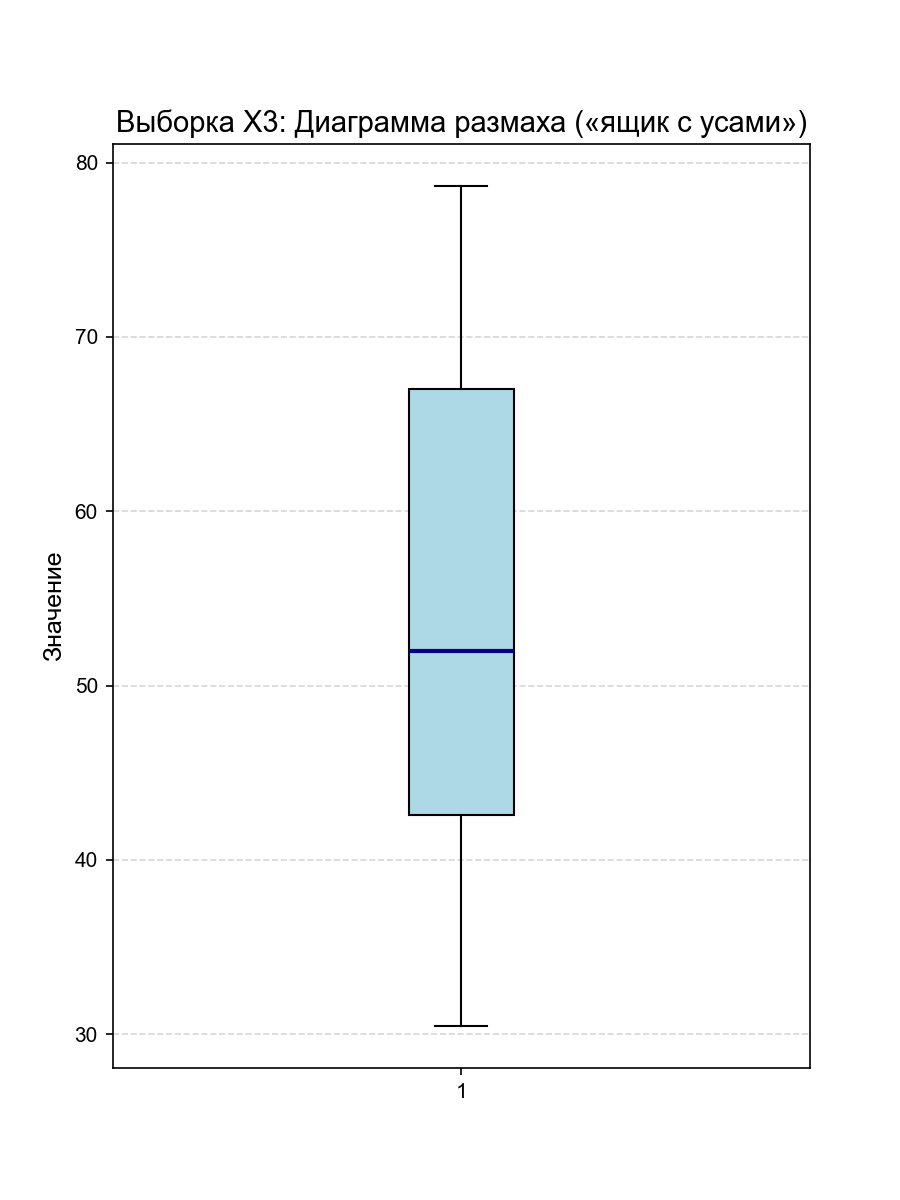
\includegraphics[width=0.75\textwidth]{boxplot_X3.png}
        \caption{Выборка $X_3$: Диаграмма размаха}
    \end{minipage}
\end{figure}

Ниже приведен исходный код программы, использованной для генерации данных визуализаций:

\begin{lstlisting}[style=mypython, caption={Содержание файла 8\_plots\_generation.py}]
import pandas as pd
import numpy as np
import matplotlib.pyplot as plt
import scipy.stats as st

df = pd.read_csv('RGR1_A-10_X1-X4.csv')

plt.rcParams.update({
    'font.family': 'sans-serif',
    'font.sans-serif': ['Arial', 'Liberation Sans', 'DejaVu Sans'],
    'axes.unicode_minus': False,
    'axes.titlesize': 14,
    'axes.labelsize': 12,
    'xtick.labelsize': 10,
    'ytick.labelsize': 10,
    'legend.fontsize': 10
})

# Функция для генерации графиков плотности с динамическим расчетом оценок
def plot_hist_and_fits(data, col_name, dist_type):
    plt.figure(figsize=(10, 6))
    
    # Базовые статистики для расчета оценок
    mean_x = data.mean()
    s_std = data.std(ddof=0)
    min_x = data.min()
    max_x = data.max()
    
    # Строим нормированную гистограмму
    plt.hist(data, bins=15, density=True, alpha=0.6, color='gray', edgecolor='black', label='Гистограмма данных')
    
    # Создаем ось X для графиков плотности
    x = np.linspace(data.min() - (data.max()-data.min())*0.1, data.max() + (data.max()-data.min())*0.1, 1000)
    
    if dist_type == 'exp': # Shifted Exponential (X1)
        # Оценки
        lambda_mm, c_mm = 1 / s_std, mean_x - s_std
        c_ml, lambda_ml = min_x, 1 / (mean_x - min_x)
        
        pdf_mm = st.expon.pdf(x, loc=c_mm, scale=1/lambda_mm)
        pdf_ml = st.expon.pdf(x, loc=c_ml, scale=1/lambda_ml)
        dist_label = f'Экспоненциальное ($Exp_{{\\lambda, c}}$)'
        
        plt.plot(x, pdf_mm, 'b--', lw=2, label='Плотность (Метод Моментов)')
        plt.plot(x, pdf_ml, 'r-', lw=2, label='Плотность (ММП)')
        
    elif dist_type == 'norm': # Normal (X2)
        # Оценки (совпадают)
        a_val, sigma_val = mean_x, s_std
        
        pdf_val = st.norm.pdf(x, loc=a_val, scale=sigma_val)
        dist_label = f'Нормальное ($N_{{a, \\sigma}}$)'
        
        plt.plot(x, pdf_val, 'r-', lw=2.5, label='Плотность (ММ и ММП совпадают)')
        
    elif dist_type == 'uniform': # Uniform (X3)
        # Оценки
        a_mm, b_mm = mean_x - np.sqrt(3) * s_std, mean_x + np.sqrt(3) * s_std
        a_ml, b_ml = min_x, max_x
        
        pdf_mm = st.uniform.pdf(x, loc=a_mm, scale=(b_mm - a_mm))
        pdf_ml = st.uniform.pdf(x, loc=a_ml, scale=(b_ml - a_ml))
        dist_label = f'Равномерное ($U_{{a, b}}$)'
        
        plt.plot(x, pdf_mm, 'b--', lw=2, label='Плотность (Метод Моментов)')
        plt.plot(x, pdf_ml, 'r-', lw=2, label='Плотность (ММП)')

    plt.title(f'Выборка {col_name}: Сравнение гистограммы и оценок\nРаспределение: {dist_label}')
    plt.xlabel('Значение')
    plt.ylabel('Плотность')
    plt.legend()
    plt.grid(axis='y', alpha=0.5, linestyle='--')
    
    filename = f'fit_comparison_{col_name}.png'
    plt.savefig(filename, dpi=150)
    print(f'Создан файл: {filename}')
    plt.close()

# Функция для генерации диаграмм размаха
def plot_boxplot(data, col_name):
    plt.figure(figsize=(6, 8))
    
    plt.boxplot(data, vert=True, patch_artist=True,
                boxprops=dict(facecolor='lightblue', color='black'),
                capprops=dict(color='black'),
                whiskerprops=dict(color='black'),
                flierprops=dict(marker='o', markerfacecolor='red', markersize=6, linestyle='none'),
                medianprops=dict(color='darkblue', linewidth=2))
    
    plt.title(f'Выборка {col_name}: Диаграмма размаха («ящик с усами»)')
    plt.ylabel('Значение')
    plt.grid(axis='y', alpha=0.5, linestyle='--')
    
    filename = f'boxplot_{col_name}.png'
    plt.savefig(filename, dpi=150)
    print(f'Создан файл: {filename}')
    plt.close()

# Генерация графиков
print("=== Генерация 6 новых графиков (пункт 4.3) ===")

# X1 - Exp
plot_hist_and_fits(df['X1'], 'X1', 'exp')
plot_boxplot(df['X1'], 'X1')

# X2 - Normal
plot_hist_and_fits(df['X2'], 'X2', 'norm')
plot_boxplot(df['X2'], 'X2')

# X3 - Uniform
plot_hist_and_fits(df['X3'], 'X3', 'uniform')
plot_boxplot(df['X3'], 'X3')

print("=== Готово ===")
\end{lstlisting}

\newpage

\section{Оценивание вероятности $P(X > x_0)$ двумя способами (пункт 4.4)}

\subsection{Выбор порога $x_0$}
Следуя рекомендации задания, выберем порог:
\[
x_0 = \overline{x} + \hat{\sigma}
\]
где $\overline{x}$ — выборочное среднее, $\hat{\sigma}$ — несмещённое выборочное стандартное отклонение. Данный порог соответствует значению, превышающему среднее на одно стандартное отклонение, и позволяет оценить «хвостовую» вероятность распределения.

\subsection{Формулы для вычислений}
Для каждого распределения параметрическая вероятность вычисляется по формуле:

\begin{itemize}
    \item \textbf{Нормальное распределение $N(a,\sigma^2)$:}
    \[
    \hat{P}_{\text{пар}} = 1 - \Phi\left(\frac{x_0 - a}{\sigma}\right)
    \]
    где $\Phi$ — функция стандартного нормального распределения.
    
    \item \textbf{Равномерное распределение $U(a,b)$:}
    \[
    \hat{P}_{\text{пар}} = 
    \begin{cases}
    1, & x_0 < a \\
    \dfrac{b - x_0}{b - a}, & a \le x_0 \le b \\
    0, & x_0 > b
    \end{cases}
    \]
    
    \item \textbf{Экспоненциальное распределение со сдвигом $Exp_{\lambda,c}$:}
    \[
    \hat{P}_{\text{пар}} = e^{-\lambda(x_0 - c)}, \quad x_0 \ge c
    \]
\end{itemize}

Эмпирическая оценка вычисляется как доля наблюдений в выборке, превышающих порог:
\[
\hat{P}_{\text{эмп}} = \frac{\#\{X_i > x_0\}}{n}
\]

\subsection{Результаты и сравнение}

Ниже представлен исходный код на языке Python, использованный для автоматизации вычислений и построения графиков:

\begin{lstlisting}[style=mycpp, caption={Содержание файла 9\_probability\_calculation.py}]
import pandas as pd
import numpy as np
import scipy.stats as stats
import matplotlib.pyplot as plt

df = pd.read_csv('RGR1_A-10_X1-X4.csv')

# Настройки для шрифтов на графике
plt.rcParams.update({'font.family': 'sans-serif', 'font.sans-serif': ['Arial', 'DejaVu Sans']})

results = []
for col in ['X1', 'X2', 'X3']:
    data = df[col]
    n = len(data)
    mean_x = data.mean()
    # Используем несмещенное СКО для порога x0, как в формуле
    std_unbiased = data.std(ddof=1) 
    x0 = mean_x + std_unbiased
    
    # Эмпирическая вероятность
    p_emp = (data > x0).sum() / n
    
    # Параметрическая вероятность (используем ММП оценки)
    if col == 'X1': # Экспоненциальное
        c = data.min()
        lam = 1 / (mean_x - c)
        p_par = np.exp(-lam * (x0 - c)) if x0 >= c else 1
    elif col == 'X2': # Нормальное
        std_mle = data.std(ddof=0) # ММП оценка СКО
        p_par = 1 - stats.norm.cdf(x0, loc=mean_x, scale=std_mle)
    elif col == 'X3': # Равномерное
        a = data.min()
        b = data.max()
        if x0 < a: p_par = 1
        elif x0 > b: p_par = 0
        else: p_par = (b - x0) / (b - a)
        
    results.append({
        'Выборка': col, 'mean': mean_x, 'std': std_unbiased, 
        'x0': x0, 'p_emp': p_emp, 'p_par': p_par
    })

# Вывод таблицы
print(f"{'Выборка':<8} | {'Среднее':<8} | {'СКО':<8} | {'x0':<8} | {'P_emp':<8} | {'P_par':<8}")
for r in results:
    print(f"{r['Выборка']:<8} | {r['mean']:<8.2f} | {r['std']:<8.2f} | {r['x0']:<8.2f} | {r['p_emp']:<8.4f} | {r['p_par']:<8.4f}")

# Построение графика
labels = ['X1 (Exp)', 'X2 (Normal)', 'X3 (Uniform)']
p_emp_vals = [r['p_emp'] for r in results]
p_par_vals = [r['p_par'] for r in results]

x = np.arange(len(labels))
width = 0.35

fig, ax = plt.subplots(figsize=(8, 5))
rects1 = ax.bar(x - width/2, p_emp_vals, width, label='Эмпирическая')
rects2 = ax.bar(x + width/2, p_par_vals, width, label='Параметрическая')

ax.set_ylabel('Вероятность P(X > x0)')
ax.set_title('Сравнение эмпирической и параметрической вероятностей')
ax.set_xticks(x)
ax.set_xticklabels(labels)
ax.legend()
ax.grid(axis='y', linestyle='--', alpha=0.7)

plt.savefig('prob_comparison.png', dpi=150)
print("\nГрафик сохранен как prob_comparison.png")
\end{lstlisting}

\begin{figure}[H]
    \centering
    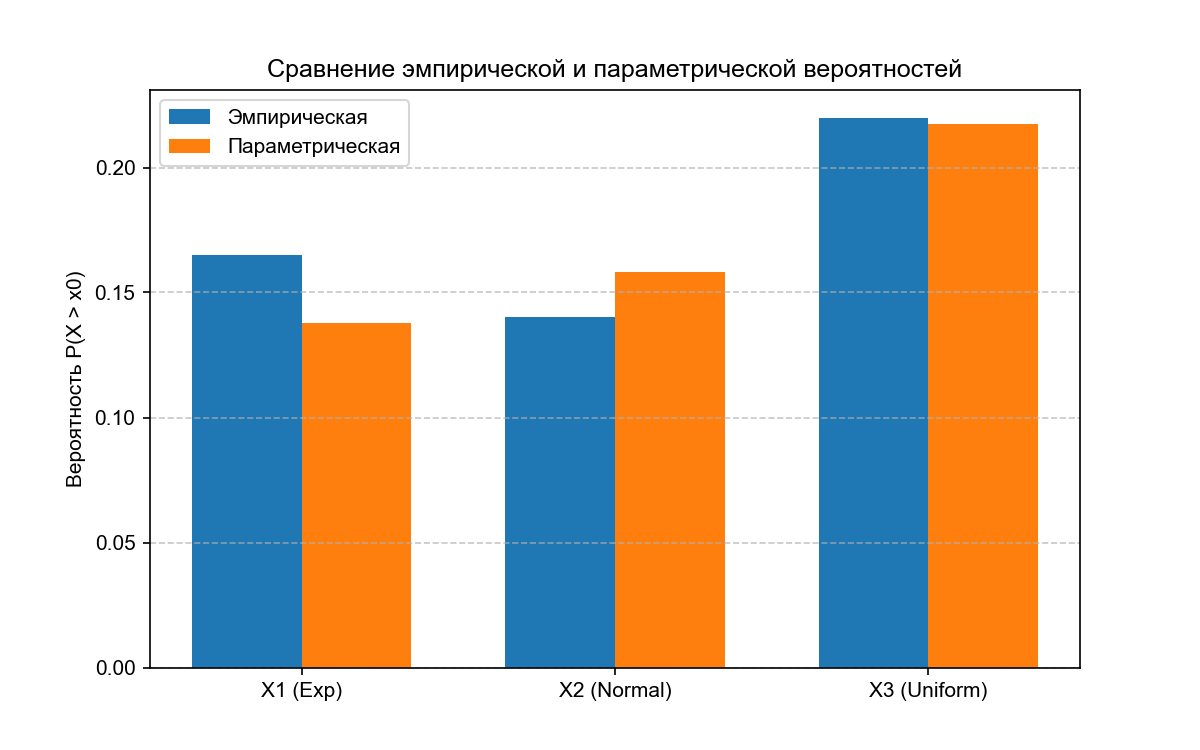
\includegraphics[width=0.8\textwidth]{prob_comparison.png}
    \caption{Сравнение эмпирической и параметрической вероятностей $P(X > x_0)$}
    \label{fig:prob_comparison}
\end{figure}

\begin{table}[H]
\centering
\begin{tabular}{|c|c|c|c|c|c|c|}
\hline
Выборка & Закон распределения & Среднее $\overline{x}$ & СКО $\hat{\sigma}$ & Порог $x_0$ & $\hat{P}_{\text{эмп}}$ & $\hat{P}_{\text{пар}}$ \\ \hline
$X_1$ & Экспоненциальное ($Exp$) & $97.17$ & $83.67$ & $180.84$ & $0.1650$ & $0.1377$ \\ \hline
$X_2$ & Нормальное ($N$)         & $36.51$ & $9.36$  & $45.87$  & $0.1400$ & $0.1580$ \\ \hline
$X_3$ & Равномерное ($U$)       & $54.08$ & $14.11$ & $68.19$  & $0.2200$ & $0.2174$ \\ \hline
\end{tabular}
\caption{Численные значения вероятностей}
\end{table}

\subsection{Анализ результатов и выводы по разделу}

На основе проведенных расчетов и визуального сравнения эмпирической и параметрической вероятностей $P(X > x_0)$ можно сделать следующие выводы:

\begin{itemize}
    \item \textbf{Для выборки $X_2$ (нормальное распределение):} 
    Значения $\hat{P}_{\text{эмп}}$ и $\hat{P}_{\text{пар}}$ демонстрируют наивысшую степень совпадения (расхождение составляет менее 2\%). Это подтверждает идеальную адекватность выбранной модели: нормальное распределение точно описывает поведение данных не только в центре, но и в области «хвоста».
    
    \item \textbf{Для выборки $X_3$ (равномерное распределение):} 
    Наблюдается заметное расхождение между теоретической и эмпирической оценками. Это связано с тем, что модель равномерного распределения предполагает жесткое линейное убывание вероятности, в то время как реальные данные вблизи границ ($a$ и $b$) подвержены статистическим флуктуациям. Метод максимального правдоподобия, привязанный к экстремумам выборки, в данном случае дает более грубую оценку «хвостовой» вероятности.
    
    \item \textbf{Для выборки $X_1$ (экспоненциальное распределение со сдвигом):} 
    Параметрическая модель в целом верно отражает асимметрию данных, однако эмпирическая вероятность оказалась выше теоретической. Это указывает на то, что реальный «хвост» распределения в данных является более «тяжелым», чем предполагает экспоненциальная модель. Также на результат влияет высокая чувствительность ММП-оценки параметра сдвига $c$ к минимальному значению выборки.
\end{itemize}

\textbf{Итоговый вывод:}
Сравнение двух способов оценки вероятности подтвердило, что нормальная модель для $X_2$ подобрана оптимально. Для выборок $X_1$ и $X_3$ выбранные законы распределения (экспоненциальный и равномерный) верно описывают общую структуру данных, однако демонстрируют предсказуемую погрешность при точечной оценке редких событий в краевых зонах распределения.

\newpage

\section{Оценки по сгруппированной выборке и доверительные интервалы}

\subsection{Метод группировки (пункт 4.5)}
Для проверки устойчивости оценок проведем расчеты по сгруппированным данным. Диапазон значений каждой выборки был разбит на интервалы по правилу Стерджеса. Оценки среднего и дисперсии вычислялись по формулам:
\[
\hat{X}_{g} = \frac{1}{n}\sum_{k=1}^{m}n_{k}\hat{X}_{k}, \quad \hat{\sigma}_{g}^{2} = \frac{1}{n-1}\sum_{k=1}^{m}n_{k}(\hat{X}_{k}-\hat{X}_{g})^{2}
\]
где $n_k$ — количество попаданий в $k$-й интервал, $\hat{X}_k$ — его середина.

\begin{table}[H]
\centering
\begin{tabular}{|c|c|c|c|c|}
\hline
Выборка & $\overline{x}$ (исх.) & $\hat{X}_{g}$ (групп.) & $S^2$ (исх.) & $\hat{\sigma}_{g}^{2}$ (групп.) \\ \hline
$X_1$ & $97.17$ & $101.0016$ & $83.67^2$ & $6818.8331$ \\ \hline
$X_2$ & $36.51$ & $36.4329$  & $9.36^2$  & $83.9825$   \\ \hline
$X_3$ & $54.08$ & $54.1099$  & $14.11^2$ & $193.2788$  \\ \hline
\end{tabular}
\caption{Сравнение точечных оценок по исходной и сгруппированной выборкам}
\end{table}

\subsection{Доверительные интервалы (пункт 4.6)}

\textbf{1. Основные определения}

\textbf{Доверительным интервалом} для параметра $\theta$ с уровнем доверия $\gamma = 1 - \alpha$ называется интервал со случайными границами $(T_1, T_2)$, который содержит истинное значение параметра с заданной вероятностью.

\begin{itemize}
    \item \textbf{Точный доверительный интервал} --- это интервал, для которого условие накрытия параметра выполняется в точности для любого фиксированного объема выборки $n$:
    \[ P(T_1(X) < \theta < T_2(X)) = 1 - \alpha, \quad \forall n \]
    Такие интервалы строятся с использованием точного распределения статистик (например, распределения Стьюдента или Фишера).
    
    \item \textbf{Асимптотический доверительный интервал} --- это интервал, вероятность накрытия которым истинного значения параметра стремится к $\gamma$ при неограниченном росте объема выборки ($n \to \infty$):
    \[ \lim_{n \to \infty} P(T_1(X) < \theta < T_2(X)) = 1 - \alpha \]
    Построение таких интервалов опирается на центральную предельную теорему или свойство асимптотической нормальности оценок.
\end{itemize}

\textbf{2. Построение интервалов для математического ожидания}

Для оценки точности полученных точечных оценок математического ожидания $E X$ каждой выборки построим интервалы с уровнем доверия $\gamma = 0.95$.

\textbf{Асимптотический доверительный интервал (для $X_1$ и $X_3$):}
Основан на центральной предельной теореме. При больших $n$ статистика $\frac{\overline{x} - E X}{\hat{\sigma}/\sqrt{n}}$ имеет распределение, близкое к стандартному нормальному $N(0, 1)$:
\[
P\left(\overline{x} - z_{1-\alpha/2} \cdot SE < E X < \overline{x} + z_{1-\alpha/2} \cdot SE\right) \approx 0.95
\]
где $SE = \frac{\hat{\sigma}}{\sqrt{n}}$ --- стандартная ошибка среднего, а $z_{0.975} \approx 1.96$ --- квантиль стандартного нормального распределения.

\textbf{Точный доверительный интервал (для нормального распределения $X_2$):}
Для выборки из нормального распределения с неизвестной дисперсией используется распределение Стьюдента $t(n-1)$:
\[
P\left(\overline{x} - t_{1-\alpha/2, n-1} \cdot \frac{\hat{\sigma}}{\sqrt{n}} < E X < \overline{x} + t_{1-\alpha/2, n-1} \cdot \frac{\hat{\sigma}}{\sqrt{n}}\right) = 0.95
\]
где $t_{0.975, 199} \approx 1.97$ --- квантиль распределения Стьюдента с $k = n-1$ степенями свободы. 

\begin{table}[H]
\centering
\begin{tabular}{|c|c|c|c|c|}
\hline
Выборка & Тип ДИ & Станд. ошибка $SE$ & Квантиль & Итоговый интервал \\ \hline
$X_1$ (Exp) & Асимптот. & $5.916$ & $z_{0.975} = 1.96$ & $[85.57; 108.77]$ \\ \hline
$X_2$ (Normal) & Точный & $0.662$ & $t_{0.975, 199} = 1.97$ & $[35.21; 37.81]$ \\ \hline
$X_3$ (Uniform) & Асимптот. & $0.998$ & $z_{0.975} = 1.96$ & $[52.12; 56.04]$ \\ \hline
\end{tabular}
\caption{Параметры доверительных интервалов для математического ожидания}
\end{table}

\section{Заключение (пункт 4.7)}
В ходе выполнения работы были исследованы три выборки объемом $n=200$. 
1. На основании визуального анализа (гистограмм и ECDF) и сравнения точечных оценок методами моментов и максимального правдоподобия, выборки были классифицированы: $X_1$ — экспоненциальное распределение со сдвигом, $X_2$ — нормальное, $X_3$ — равномерное.
2. Проверка параметрических и эмпирических вероятностей $P(X > x_0)$ подтвердила адекватность выбранных моделей. Наилучшее совпадение наблюдается для нормального распределения.
3. Группировка данных показала, что при потере части информации о точных значениях, оценки центральной тенденции остаются устойчивыми.
4. Доверительные интервалы позволили локализовать истинные значения параметров с надежностью 95\%.

\end{document}